\documentclass[12pt,a4paper]{article}
\usepackage{amsmath}
\usepackage{fixltx2e}
\usepackage{ifthen}
\usepackage{etoolbox}
\usepackage{xcolor}
\usepackage{tikz}
\usepackage[none]{hyphenat}

\usetikzlibrary{backgrounds,calc,through,positioning,arrows,automata}
\begin{document}

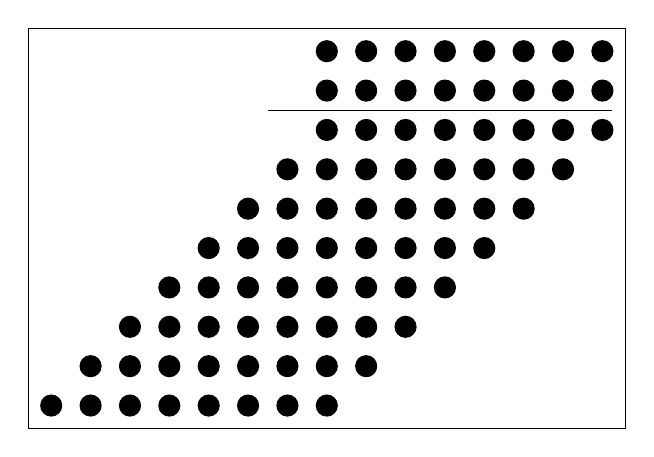
\begin{tikzpicture}[scale=0.5,show background rectangle]]
\tikzstyle{every node}=[fill,shape=circle,minimum width=8pt, inner sep=0pt];

\foreach \i in {10,...,17} {
	\node at (\i,10.5) {}; %operand a
	\node at (\i,9.5) {}; %operand b
}
	\draw (8.5,9) -- (17.25,9);

\foreach \i in {1,...,8} {
	\foreach \j in {1,...,8} {
		\node at (\i+\j+1,\j+0.5) {}; %operand a
	}
}
\end{tikzpicture}

\vspace{5cm}

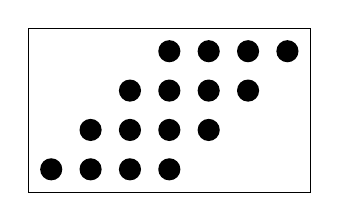
\begin{tikzpicture}[scale=0.5,show background rectangle]]
\tikzstyle{every node}=[fill,shape=circle,minimum width=8pt, inner sep=0pt];

\foreach \i in {1,...,4} {
	\foreach \j in {1,...,4} {
		\node at (\i+\j+1,\j+0.5) {}; %operand a
	}
}
\end{tikzpicture}

\vspace{5cm}



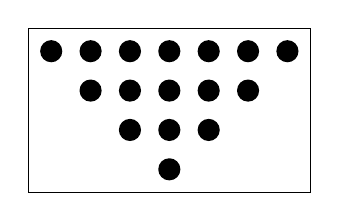
\begin{tikzpicture}[scale=0.5,show background rectangle]]
\tikzstyle{every node}=[fill,shape=circle,minimum width=8pt, inner sep=0pt];
% \draw[step=1,gray,very thin] (0,0) grid (5,5);

\foreach \j in {1,...,7} {
	\node at (\j,5) {};
	\ifthenelse{\j>1 \AND \j<7}{\node at (\j,4) {};}{}
	\ifthenelse{\j>2 \AND \j<6}{\node at (\j,3) {};}{}
	\ifthenelse{\j>3 \AND \j<5}{\node at (\j,2) {};}{}
	\ifthenelse{\j>4 \AND \j<4}{\node at (\j,1) {};}{}
	\ifthenelse{\j>5 \AND \j<3}{\node at (\j,0) {};}{}
		% 	% }{%
		% 	% 	\node [red] at (\i+\j+1,\j+0.5) {};
		% 	% }%
		% }%
}

\end{tikzpicture}

\vspace{5cm}

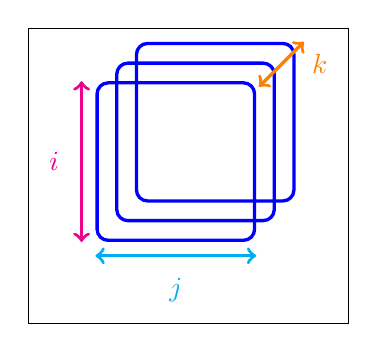
\begin{tikzpicture}[scale=1,show background rectangle]]

% \draw[step=0.25,gray,very thin] (-2,-2) grid (3.5,3.5);

\tikzstyle{mybox} = [fill=none, very thick, rectangle, rounded corners, minimum height=2cm,minimum width=2cm]

\node (c3) [mybox,draw=blue] at (0.5,0.5) {};
\node (c2) [mybox,draw=blue] at (0.25,0.25) {};
\node (c1) [mybox,draw=blue] at (0,0) {};

\draw[orange,very thick,<->] (c1.north east)+(1pt,-2pt) -- ($(c3.north east)+(3pt,0pt)$)  node (k) [pos=.5,right=0.25cm] {$k$};
\draw[cyan,very thick,<->] (c1.south west)+(0,-5pt) -- ($(c1.south east)+(0,-5pt)$)  node (k) [pos=.5,below=0.15cm] {$j$};
\draw[magenta,very thick,<->] (c1.north west)+(-5pt,0pt) -- ($(c1.south west)+(-5pt,0)$)  node (k) [pos=.5,left=0.15cm] {$i$};

\end{tikzpicture}


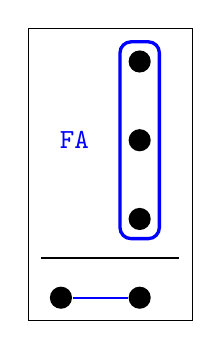
\begin{tikzpicture}[scale=1,show background rectangle]]

% \draw[step=0.25,gray,very thin] (-2,-3) grid (2,5);

\tikzstyle{mybox} = [fill=none, very thick, rectangle, rounded corners, minimum height=2.5cm,minimum width=0.5cm]
\tikzstyle{mydot}=[fill,shape=circle,minimum width=8pt, inner sep=0pt];

\node (fa) [mybox,draw=blue] at (0,1) {};
\node (fatext) [blue,left=0.25cm of fa] {\texttt{FA}};

\node [mydot] (n1) at (0,0) {};
\node [mydot] (n2) at (0,1) {};
\node [mydot] (n3) at (0,2) {};
\draw [black,thick] (n1)+(-1.25cm,-0.5cm) -- ($(n1)+(0.5cm,-0.5cm)$);

\node [mydot] (s) at ($(n1)+(0,-1)$) {};
\node [mydot] (cout) at ($(s)+(-1,0)$) {};
\draw [blue,thick] (s) -- (cout);

\end{tikzpicture}

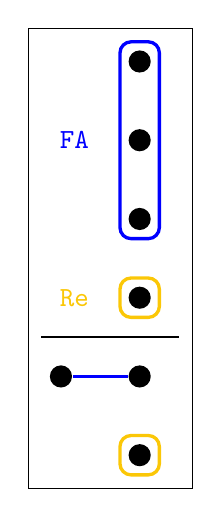
\begin{tikzpicture}[scale=1,show background rectangle]]

% \draw[step=0.25,gray,very thin] (-2,-3) grid (2,5);

\tikzstyle{mybox} = [fill=none, very thick, rectangle, rounded corners, minimum height=2.5cm,minimum width=0.5cm]
\tikzstyle{mydot}=[fill,shape=circle,minimum width=8pt, inner sep=0pt];

\node (fa) [mybox,draw=blue] at (0,2) {};
\node (fatext) [blue,left=0.25cm of fa] {\texttt{FA}};
\node (re) [mybox,minimum height=0.5cm,draw=yellow!80!red] at (0,0) {};
\node (retext) [blue,yellow!80!red,left=0.25cm of re] {\texttt{Re}};

\node [mydot] (n1) at (0,0) {};
\node [mydot] (n2) at (0,1) {};
\node [mydot] (n3) at (0,2) {};
\node [mydot] (n4) at (0,3) {};
\draw [black,thick] (n1)+(-1.25cm,-0.5cm) -- ($(n1)+(0.5cm,-0.5cm)$);

\node [mydot] (s1) at ($(n1)+(0,-1)$) {};
\node [mydot] (cout) at ($(s1)+(-1,0)$) {};
\draw [blue,thick] (s1) -- (cout);

\node (re2) [mybox,minimum height=0.5cm,draw=yellow!80!red] at (0,-2) {};
\node [mydot] (s2) at ($(s1)+(0,-1)$) {};

\end{tikzpicture}


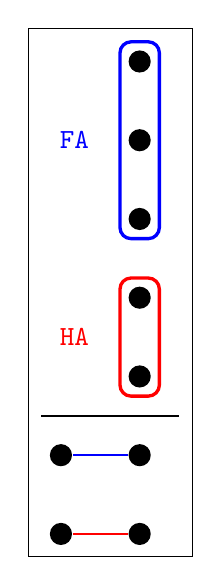
\begin{tikzpicture}[scale=1,show background rectangle]]

% \draw[step=0.25,gray,very thin] (-2,-3) grid (2,5);

\tikzstyle{fabox} = [fill=none, very thick, draw=blue, rectangle, rounded corners, minimum height=2.5cm,minimum width=0.5cm]
\tikzstyle{habox} = [fill=none, very thick, draw=red, rectangle, rounded corners, minimum height=1.5cm,minimum width=0.5cm]
\tikzstyle{mydot}=[fill,shape=circle,minimum width=8pt, inner sep=0pt];

\node (fa) [fabox] at (0,3) {};
\node (fatext) [blue,left=0.25cm of fa] {\texttt{FA}};
\node (ha) [habox] at (0,0.5) {};
\node (hatext) [red,left=0.25cm of ha] {\texttt{HA}};

\node [mydot] (n1) at (0,0) {};
\node [mydot] (n2) at (0,1) {};
\node [mydot] (n3) at (0,2) {};
\node [mydot] (n4) at (0,3) {};
\node [mydot] (n5) at (0,4) {};
\draw [black,thick] (n1)+(-1.25cm,-0.5cm) -- ($(n1)+(0.5cm,-0.5cm)$);

\node [mydot] (s1) at ($(n1)+(0,-1)$) {};
\node [mydot] (cout1) at ($(s1)+(-1,0)$) {};
\draw [blue,thick] (s1) -- (cout1);

\node [mydot] (s2) at ($(n1)+(0,-2)$) {};
\node [mydot] (cout2) at ($(s2)+(-1,0)$) {};
\draw [red,thick] (s2) -- (cout2);

\end{tikzpicture}


\def\myscale{1}

\tikzset{% 
	inputport/.style={very thick, color=green!60!black},
	outputport/.style={very thick, color=red!80!black}
}

\begin{tikzpicture}[scale=\myscale,show background rectangle]]

\tikzstyle{mybox} = [draw=gray!50, fill=gray!5, very thick, rectangle, rounded corners, minimum height=\myscale*4cm,minimum width=\myscale*3cm]
\node [mybox] (box) at (3,3.5) {%
	\begin{minipage}{0.2\textwidth}
	\centering 
	\texttt{mul32}\\[0.3cm]
	\textbf{generics:}\\
	\ttfamily tech\\multype\\pipe\\mac
	\end{minipage}
};


\draw[inputport, -|] (0,5) -- ++(1.5,0) node (rst) [pos=.5,above] {\texttt{rst}};
\draw[inputport, -|] (0,4) -- ++(1.5,0) node (clk) [pos=.5,above] {\texttt{clk}};
\draw[inputport, -|] (0,3) -- ++(1.5,0) node (holdn) [pos=.5,above] {\texttt{holdn}};
\draw[inputport, -|] (0,2) -- ++(1.5,0) node (muli) [pos=.5,above] {\texttt{muli}};

\draw[very thick, outputport, |-] (4.5,5) -- ++(1.5,0) node (mulo) [pos=.5,above] {\texttt{mulo}};


% \node (input)  [inputport, above=0.25cm of rst] {\textbf{Input}};
% \node (mul)    [color=black, above=0.35cm of box] {\textbf{mul32}};
% \node (output) [outputport, above=0.25cm of mulo] {\textbf{Output}};

\end{tikzpicture}

\vspace{5cm}

\begin{tikzpicture}[show background rectangle, node distance=3cm]
\node (muli) [inputport, anchor=west] at (0,0) {\texttt{muli}};
\node (op1) [inputport, anchor=west] at ++(3,0) {\texttt{op1}};
\node (op2) [inputport, anchor=west] at ++(3,-1) {\texttt{op2}};
\node (flush) [inputport, anchor=west,] at ++(3,-2) {\texttt{flush}};
\node (issigned) [inputport, anchor=west,] at ++(3,-3) {\texttt{is\_signed}};
\node (start) [inputport, anchor=west,] at ++(3,-4) {\texttt{start}};
\node (mac) [inputport, anchor=west,] at ++(3,-5) {\texttt{mac}};
\node (acc) [inputport, anchor=west,] at ++(3,-6) {\texttt{acc}};

\draw [inputport,-|](muli) -- coordinate(m1) (op1);
\draw [inputport,-|](m1) |-  (op2);
\draw [inputport,-|](m1) |- (flush);
\draw [inputport,-|](m1) |- (issigned);
\draw [inputport,-|](m1) |- (start);
\draw [inputport,-|](m1) |- (mac);
\draw [inputport,-|](m1) |- (acc);

\end{tikzpicture}

\vspace{5cm}

\begin{tikzpicture}[show background rectangle, node distance=3cm]
\node (mulo) [outputport, anchor=west,] at (0,0) {\texttt{mulo}};
\node (nready) [outputport, anchor=west] at ++(3,0) {\texttt{nready}};
\node (ready) [outputport, anchor=west] at ++(3,-1) {\texttt{ready}};
\node (icc) [outputport, anchor=west,] at ++(3,-2) {\texttt{icc}};
\node (result) [outputport, anchor=west,] at ++(3,-3) {\texttt{result}};

\draw [outputport,-|](muli) -- coordinate(m1) (nready);
\draw [outputport,-|](m1) |-  coordinate(m2) (ready);
\draw [outputport,-|](m1) |- (icc);
\draw [outputport,-|](m1) |- (result);

\end{tikzpicture}


\vspace{5cm}

\begin{tikzpicture}[scale=\myscale,show background rectangle]]

\tikzstyle{mybox} = [draw=gray!50, fill=gray!5, very thick, rectangle, rounded corners, minimum height=\myscale*3cm,minimum width=\myscale*2.5cm]
% \draw[step=0.5,black,thin] (0,0) grid (5,5);

\node [mybox] (box) at (3,2.5) {\texttt{FA}};

\draw[inputport, -|] (0.25,3.5) -- ++(1.5,0) node (x) [pos=.5,above] {\texttt{x}};
\draw[inputport, -|] (0.25,2.5) -- ++(1.5,0) node (y) [pos=.5,above] {\texttt{y}};
\draw[inputport, -|] (0.25,1.5) -- ++(1.5,0) node (cin) [pos=.5,above] {\texttt{c\textsubscript{in}}};

\draw[outputport, |-] (4.25,3) -- ++(1.5,0) node (mulo) [pos=.5,above] {\texttt{s}};
\draw[outputport, |-] (4.25,2) -- ++(1.5,0) node (mulo) [pos=.5,above] {\texttt{c\textsubscript{out}}};

\end{tikzpicture}


\vspace{5cm}

\begin{tikzpicture}[scale=\myscale,show background rectangle]]

\tikzstyle{mybox} = [draw=gray!50, fill=gray!5, very thick, rectangle, rounded corners, minimum height=\myscale*2cm,minimum width=\myscale*2cm]
% \draw[step=0.5,black,thin] (0,0) grid (5,5);

\node [mybox] (box) at (2.5,1.5) {\texttt{HA}};

\draw[inputport, -|] (0,2) -- ++(1.5,0) node (x) [pos=.5,above] {\texttt{x}};
\draw[inputport, -|] (0,1) -- ++(1.5,0) node (y) [pos=.5,above] {\texttt{y}};

\draw[outputport, |-] (3.5,2) -- ++(1.5,0) node (mulo) [pos=.5,above] {\texttt{s}};
\draw[outputport, |-] (3.5,1) -- ++(1.5,0) node (mulo) [pos=.5,above] {\texttt{c\textsubscript{out}}};

\end{tikzpicture}



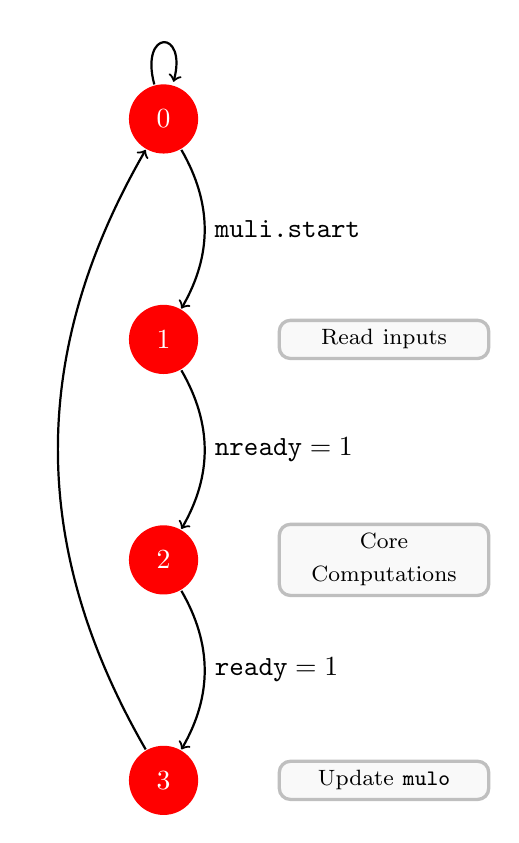
\begin{tikzpicture}[->,auto,node distance=2.8cm,thick]
	\tikzstyle{every state}=[fill=red,draw=none,text=white]

	\node[state] (A)						{$0$};
	\node[state]         (B) [below of=A]	{$1$};
	\node[state]         (C) [below of=B]	{$2$};
	\node[state]         (D) [below of=C]	{$3$};

	\path (A) edge [bend left] node [right]{\texttt{muli.start}} (B)
		  (A) edge [loop above] node [right] {} (A)
		  (B) edge [bend left] node [right]{$\text{\texttt{nready}} = 1$} (C)
		  (C) edge [bend left] node [right]{$\text{\texttt{ready}} = 1$} (D)
		  (D) edge [bend left] node [left]{} (A);


	\tikzstyle{mybox} = [draw=gray!50, fill=gray!5, very thick, rectangle, rounded corners,text width=0.20\textwidth,align=center]
	\node [mybox,right of=B] (boxB){%
		\footnotesize
		Read inputs
	};

	\node [mybox,right of=C] (boxC){\footnotesize Core Computations};

	\node [mybox,right of=D] (boxD){%
		\footnotesize
		Update \texttt{mulo}
	};

\end{tikzpicture}


\end{document}